\documentclass{article}

\PassOptionsToPackage{numbers,sort&compress}{natbib}
\usepackage[sglblindworkshop]{neurips_2026}
\workshoptitle{Machine Learning for Systems}
\usepackage[utf8]{inputenc}
\usepackage[T1]{fontenc}
\usepackage{amsmath,amssymb,amsthm}
\usepackage{booktabs}
\usepackage{graphicx}
\usepackage{microtype}
\usepackage{xcolor}
\usepackage{xspace}
\usepackage[hidelinks]{hyperref}

% The 2026 style currently emits its generic main-conference notice even for
% the single-blind workshop option. Preserve its geometry and line-number mode
% while naming the actual venue.
\makeatletter
\renewcommand{\@noticestring}{Submitted to the NeurIPS 2026 Workshop on Machine Learning for Systems.}
\makeatother

\graphicspath{{../../figures/}}
\newcommand{\dhat}{\hat{\Delta}}
\newcommand{\pizero}{\pi_0}
\newcommand{\rmax}{r_{\max}}
\newcommand{\system}{\textsc{Bouncer}\xspace}

\title{Bouncer: Runtime Competence Auditing for Partition-Local Learned Controllers}
\author{Kabir Grewal \\
  \texttt{ska@unc.edu}}

\begin{document}
\maketitle

\begin{abstract}
Learned systems controllers can beat fixed heuristics in validation yet regress
after workload shift.  Feature and confidence monitors do not directly answer
the operational question: is the learned policy still better than its fallback?
\system concurrently assigns sampled resource partitions to each policy and
gates the remaining partitions from their measured reward difference.  Its
interpretation requires representative sampling, partition-local reward, and a
policy contrast that survives assignment.  In controlled trace replay, a fitted
cache-insertion policy validates at 96.3\%, then loses to LRU after PC/reuse
semantics change while both the PC and model-confidence distributions remain
exactly fixed.  Under Zipf traffic and a hot-set-correlated shift, uniform
leaders estimate the wrong sign and detect 4/12 runs; pre-shift activity strata
reduce mean bias from $+0.247$ to $-0.0006$ and detect 12/12.  An evidence-adaptive
audit uses 2.03 rather than eight leaders per arm in the clean cell while matching
or improving detection in the tested shifts.  For a counter-like stateful policy,
shadow-updated metadata preserves a $0.298$ gap that rotation with reset attenuates
to $0.015$.  Steady-state retention and recovery equal the $7/8$
leader-allocation ceiling by design.  These are controlled mechanism repairs,
not application-level or RTL validation.
\end{abstract}

\section{Why monitor competence?}

Learned cache replacement, prefetching, memory scheduling, and branch prediction
can beat hand-designed policies by adapting to workload structure
\citep{ipek2008selfoptimizing,liu2020imitationcache,bera2021pythia,jain2016hawkeye,shi2019glider}.
Frameworks such as Park and SmartChoices make learned decisions available across
systems domains \citep{mao2019park,carstens2023smartchoices}.  Their deployed
advantage is nevertheless conditional: a model trained on one program or phase
may become worse than the heuristic it displaced.  This is a systems-specific
instance of post-deployment model debt \citep{sculley2015technicaldebt}.
Aggregate counters show that performance changed, but not whether the learned
policy caused the change.  Feature-based out-of-distribution (OOD) detection is
also indirect: a concept shift can preserve the monitored marginal while
reversing which action is useful
\citep{hendrycks2017baseline,gama2014survey,rabanser2019failing}.

Suppose a learned controller $C$ has a vetted fallback $\pizero$.  For audit
window $w$, define the competence advantage
\begin{equation}
  \Delta_w = \bar r_w^C-\bar r_w^{\pizero}, \qquad r\in[0,\rmax],
  \label{eq:competence}
\end{equation}
where reward is the system outcome attributable to a decision, such as a cache
hit.  We want to deploy $C$ while $\Delta_w\ge\tau$ and otherwise fall back.  The
counterfactual is unavailable: one physical decision cannot simultaneously run
both policies.

Under the sampling and attribution conditions below, this is an online
causal-comparison problem rather than confidence calibration.  A useful mechanism
must compare policies under concurrent traffic and state when its sample ceases
to represent deployed decisions.
\begin{minipage}{\linewidth}
\paragraph{Contributions.} We (i) define realized competence and its validity
conditions; (ii) predict finite-population leader coverage and expose a traffic-
weighted sampling failure; (iii) repair that failure with stratified estimation,
adapt audit allocation to evidence, and preserve counter-like policy state with
shadow metadata; and (iv) characterize one fitted controller across shift
severity, rate, and PSEL references.  All seeds remain synthetic-family repeats;
ChampSim remains boundary evidence.
\end{minipage}

\begin{figure}[t]
  \centering
  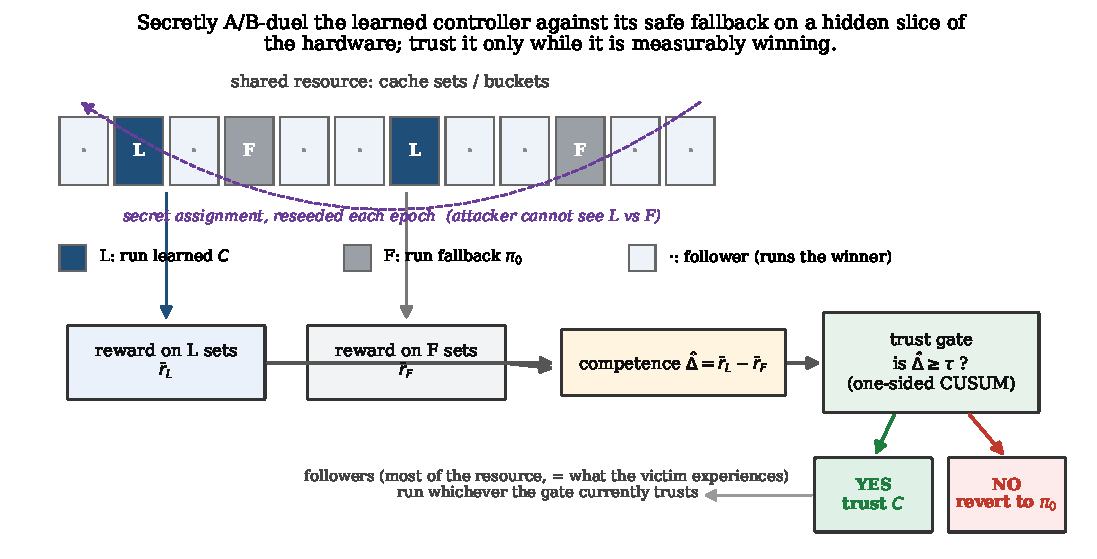
\includegraphics[width=0.85\linewidth]{concept.pdf}
  \caption{DIP topology with an explicit learned-minus-fallback estimand, gate,
  and validity conditions.  Fixed leaders preserve state; hiding and reseeding
  are outside this benign-shift study.}
  \label{fig:concept}
\end{figure}

\section{Concurrent partition A/B auditing}

\paragraph{Estimator and gate.}
\system repurposes hardware set dueling \citep{qureshi2007dip}.  It assigns
$n_C$ cache sets to $C$, $n_F$ to $\pizero$, and the rest to a follower
pool (Figure~\ref{fig:concept}).  Unlike a global before/after comparison, both
leaders observe the same concurrent workload.  Their measured difference
\begin{equation}
  \dhat_w=\bar r_{C,w}-\bar r_{F,w}
\end{equation}
feeds a lower CUSUM $S_w=\max\{0,S_{w-1}+K-\dhat_w\}$, which gates followers when
$S_w>H$ \citep{page1954cusum}.  Leaders remain policy-fixed so both arms stay
observable.  The longer artifact evaluates hysteresis and measured re-trust;
the trained study here uses a one-way gate.

Let $\Delta_w^{\rm fol}$ be the decision-weighted advantage that the follower
pool would experience.  The estimator obeys
$\mathbb E[\dhat_w\mid\mathcal H_{w-1}]=\Delta_w^{\rm fol}+b_w$.  Here
$b_{\rm sample}$ is leader/follower traffic mismatch, $b_{\rm local}$ is reward
credited outside the sampled partition, and $b_{\rm state}$ is policy-contrast
distortion caused by assignment; $b_w$ is their sum.  CUSUM controls fluctuation
around this expectation but cannot repair bias.

\paragraph{When does the comparison mean what it says?}
Three conditions are load-bearing.  \textbf{Representative sampling} requires
the leader estimate to target decision-weighted follower traffic.
\textbf{Set-locality} requires a decision and credited reward to share the
sampled partition; replacement hits satisfy this, whereas a prefetch initiated
in one set can benefit another.  \textbf{Assignment-identifiability} requires the
policy contrast to survive leader assignment.  A stateless controller satisfies
this immediately.  A stateful controller instead needs persistent leaders,
shadow-updated state, or a warm-up quarantine.  Reshuffling that repeatedly
cold-starts one arm can erase the very contrast being measured.
For the homogeneous audit, simulator-only shadow replay recomputes both policies
on every follower access without changing routing; their difference supplies
$\Delta_w^{\rm fol}$.  Against that target, mean $b_w=-0.0003$ and RMSE is
$0.0104$.  A Zipf/correlated-shift negative control instead reverses the estimand
sign and is detected in only 4/12 runs.  Thus $b_w\approx0$ is scoped to the
sampling design, not supplied by CUSUM.

\paragraph{Traffic and state repairs.}
Let pre-shift activity define strata $h$ and let $q_{h,w}$ be each stratum's
fraction of follower requests.  We estimate
$\dhat_w^{\rm strat}=\sum_hq_{h,w}(\bar r^C_{h,w}-\bar r^F_{h,w})$, placing both
policy arms in every represented stratum.  This targets request-weighted
followers when leader outcomes are representative within strata; it does not
repair unmeasured within-stratum heterogeneity.  To reduce clean-regime audit
cost, a separate stateless experiment rotates two leaders/arm through a fixed
eight-candidate cohort, expands to eight when $S_w\ge.03$ or $\dhat_w<.04$, and
shrinks after four stable windows.  Rotation is unsafe for stateful policies
unless state is preserved.  Our controlled state repair advances one small
per-policy counter for every set-window, including the inactive policy, then
restores that shadow counter on reassignment; it does not duplicate cache data.

\paragraph{Expected-cost accounting.}
Over $T$ windows,
partition regret into (i) fully open harmful windows, (ii) the learned-policy
exposure retained for auditing after gating, and (iii) false-alarm switching.
If there are $N_{\rm ep}$ harmful episodes of total duration $T_{\rm harm}$,
the expected fully open count per episode is at most $D$,
each set is exposed after gating with marginal probability at most $\phi$, the
false-alarm probability per window is at most $\alpha$, and each false-alarm
episode costs at most $c_{\rm sw}$, then
\begin{equation}
 \mathbb E[R_T]\le N_{\rm ep}D\rmax+\phi T_{\rm harm}\rmax
             +\alpha T c_{\rm sw}.                          \label{eq:floor}
\end{equation}
This expectation-level accounting is conditional on the stated inputs; it
does not make a pointwise safety claim.  In particular, $D$ is an assumed or
separately calibrated detection bound, not a latency predicted by the inequality,
and biased leaders invalidate its interpretation.  Appendix~\ref{app:theory}
gives the proof skeleton.  It does not predict $D$ or calibrate $\alpha$ from
$(K,H)$ for this stateful estimator.

\section{A trained controller under graded shift}

A four-PC logistic model predicts reuse within 64 references, inserts predicted
reusable lines, and bypasses predicted streams; true LRU is the fallback.  Labels
come from independent seeded training (20,000) and validation (5,000) traces.
Validation accuracy is 96.28\% versus a 50.82\% majority baseline, with 0.1603
log loss.  Deployment uses 64 eight-way sets, 64 accesses/set-window, and eight
fixed leaders per arm.  Every PC occurs exactly 25\% of the time in every
set-window, so both the PC histogram and any deterministic PC-only model-score
distribution have total-variation distance zero throughout.

The original 60-window maximal reversal changes all sets at window 30.  We add
an 80-window characterization that changes a nested random fraction $p$ of sets
at window 20, plus a 16-window ramp.  $K=0.02$, $H=0.12$, leader counts, and 12
seeds are fixed across cells.  Seeds change leader placement, affected sets, and
access order inside one synthetic family; these are not applications.

\begin{figure}[t]
  \centering
  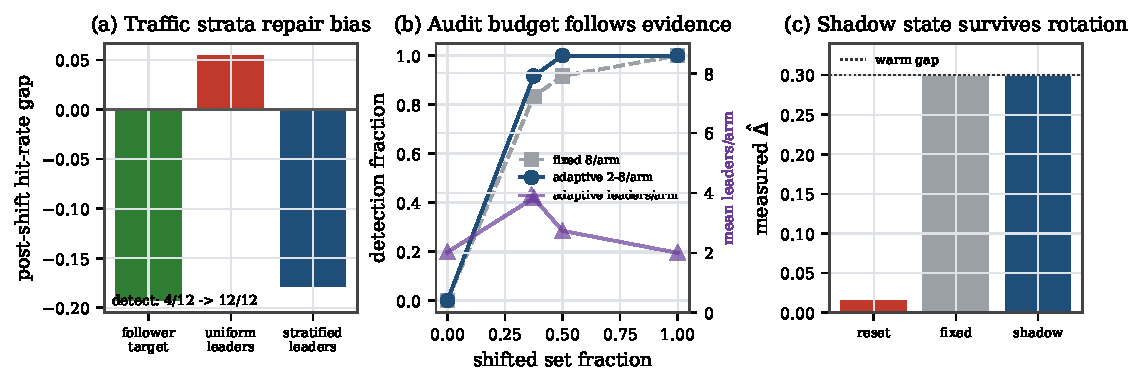
\includegraphics[width=\linewidth]{trained_upgrades.pdf}
  \caption{Three controlled repairs. (a) Request-weighted activity strata repair
  the sign error from uniform leaders. (b) A 2--8 leader/arm audit spends evidence
  where it is needed; points are 12-run detection fractions. (c) For a
  counter-like warm-up model, shadow metadata preserves the policy contrast
  under rotation.}
  \label{fig:trained}
\end{figure}

At $p=1$, learned/LRU/\system hit rates change from
$0.4375/0.3276/0.4237$ to $0/0.3279/0.2869$ and all runs gate one window later.
The 87.5\% retention and recovery are therefore the expected $7/8$ allocation
ceiling: before gating eight fallback leaders cannot earn learned gain; afterward
eight learned leaders retain exposure.  The severity sweep is nontrivial:
$p=0.375$ gates 10/12 runs (mean gap $-0.054$), $p=0.5$ gates 11/12
($-0.109$), and $p\ge0.625$ gates 12/12.  At $p=0.125$ the gap remains $+0.055>K$
yet one run-level alarm occurs over 960 in-control run-windows.  Dependence and
the latching gate make this a stress count, not an estimate of the per-window
$\alpha$ in Equation~\ref{eq:floor}.

\paragraph{Finite-population coverage.}
At $p=.25$, if $X$ is the number of shifted learned leaders then
$X\sim\mathrm{Hypergeom}(64,16,8)$, not eight independent coin flips.
$\mathbb E[X]=2$ and overlap alone predicts leader-gap standard deviation .063,
close to .066 measured across seeds.  It predicts a .649 one-window probability
of falling below $K$; the full stateful rule gates 7/12, versus 3/12 for both
PSEL widths.  Among PSEL detections, delay is 4.33 windows at 8 bits and 15.33 at
10 bits.  The deterministic $H/(K-\mathbb E[\dhat])$ heuristic gives 6.08 windows
versus \system's observed 4.14 among detections, within a factor 1.47 but not a
calibration guarantee.  The 16-window full ramp gates 12/12 in 4.75 windows after
the same three-window mean gap-crossing event used for every reference rule.

\paragraph{Repair results.}
In the Zipf-1.2 control, the hottest eighth holds 68.2\% of request mass and is
the only shifted stratum.  Uniform leaders target sets rather than follower
requests: the true follower gap is $-0.193$, but $\dhat=+0.055$ (mean bias
$+0.247$), yielding 4/12 detections.  Assigning one leader/arm to the hot
stratum and seven to the cold stratum, then weighting stratum contrasts by
follower request mass, gives target $-0.178$, estimate $-0.179$, bias $-0.0006$,
and 12/12 detections.  This repairs this known two-stratum construction only.
The adaptive audit averages 2.03 leaders/arm with no clean alarms, versus eight
fixed, and detects 11/12 versus 10/12 at $p=.375$, 12/12 versus 11/12 at $p=.5$,
and 12/12 at $p=1$ using two.  Finally, at a 20-window warm-up timescale,
resetting state yields $\dhat=.015$ for a true .300 gap; fixed leaders and two
8-bit shadow counters/set recover .299 and .298.  The modeled metadata is 128 B
for 64 sets (4 KiB for 2048), not an RTL or cache-content implementation.

\section{Broader evidence and boundaries}

The trained case complements, rather than replaces, the artifact's broader
tests.  In the seeded competence harness, $\dhat$ tracks known ground truth
($R^2=0.997$); the released operating point gates in two windows, limits the
worst attacked steady window to 0.64\% below the fallback, and detects 50/50
input-mimicry attacks while an input-OOD monitor detects 0/50.  These are
synthetic mechanism tests with explicit reward models.

The ChampSim integration supplies boundary evidence, not a clean win.  On one
SPEC 623.xalancbmk trace, the LLC candidate is LIP insertion at RRPV 3 and the
fallback is SRRIP-HP insertion at RRPV 2; these are hand-designed policies, not
the fitted controller above.  Their whole-cache hit rates are 0.336/0.048, yet
leader reassignment attenuates mean $\dhat$ to 0.005; fixed leaders recover 0.23.
Prefetch reward is also nonlocal.  These one-trace, one-seed measurements show
why assignment-identifiability and locality are premises, not generalization.
Neither study measures RTL area, energy, timing, or silicon; a 406-byte state
proposal is not a synthesis result.

\section{Related work and positioning}
Learned cache, prefetch, and scheduling policies show fitted controllers can beat
heuristics \citep{ipek2008selfoptimizing,bera2021pythia,jain2016hawkeye,
shi2019glider,liu2020imitationcache}; \system instead audits a candidate that
already exists.  OOD monitors detect changed inputs
\citep{hendrycks2017baseline,gama2014survey}; we compare local rewards.  A/B
testing shares that goal \citep{kohavi2009controlled}, while partition leaders
avoid cross-window stability (the temporal diagnostic costs 50\% exposure).
Simplex and safe improvement offer stronger guarantees
\citep{sha2001simplicity,thomas2015hcpi}.  We reuse DIP's substrate
\citep{qureshi2007dip,jaleel2010rrip} with an explicit estimand and CUSUM gate
\citep{page1954cusum}; no sequential rule repairs biased sampling.

\section{Limitations and conclusion}

The controller and shift are constructed; 12 seeds cover one family, hit rate is
not IPC, and $(K,H)$ is uncalibrated.  The stratified repair is narrow, adaptive
rotation is stateless, and shadow counters are not cache contents.  \system cannot
audit nonlocal reward or destroyed contrasts.  Within scope, 61 checks reproduce
marginal-invisible reversals and failures; application and hardware validation
remain future work.

\clearpage
\bibliographystyle{plainnat}
\bibliography{../references}

\clearpage
\appendix
\section{Trained-controller protocol}
\label{app:protocol}

The released scripts \texttt{exp\_trained\_controller.py} and
\texttt{exp\_trained\_characterization.py} own the original maximal demonstration
and graded-shift studies; \texttt{exp\_trained\_upgrades.py} and
\texttt{exp\_warmup\_predictor.py} own the three repairs.  The model is a
regularized binary logistic regressor
with an intercept and four one-hot PC features.  Full-batch gradient descent runs
for 800 steps at learning rate 0.4 with $10^{-3}$ weight decay.  Training traces
contain equal numbers of recurring and one-shot references; 3\% of examples cross
the usual PC/reuse association.  A label is one exactly when the same tag appears
within the next 64 references.  Training and validation traces use different
seeds.

Deployment uses a set-associative trace replay with true LRU ordering.  On a
miss, the learned policy inserts the line if its fitted reuse probability is at
least 0.5 and otherwise bypasses it.  The fallback always inserts.  Hot and
stream references are balanced, as are all four PC classes.  The PC classes
associated with hot and stream references exchange at window 30 in the original
60-window maximal protocol.  The characterization and repair protocols use 80
windows, shift a nested fraction of sets at window 20, and discard the first eight
post-shift windows when reporting steady state.  The original protocol is exactly
the $p=1$ endpoint under the earlier timing.  Hot tags rotate each window,
preventing the learned controller from coasting indefinitely on state established
before the shift.

Each evaluation seed draws one fixed partition: eight learned leaders,
eight fallback leaders, and 48 followers.  The one-sided lower CUSUM uses
$K=0.02$ and $H=0.12$.  Evidence from window $w$ changes follower routing at
window $w+1$, so the reported one-window delay is causal rather than same-window
routing.  The maximal experiment asserts detection in every seed; the severity
sweep records misses and gates without filtering.  The JSON and all manuscript
numbers are checked by \texttt{scripts/check\_ml4sys\_numbers.py}.  Seed-level
intervals use the two-sided Student-$t$ critical value 2.200985 for 11 degrees of
freedom; no application-level population inference is intended.

The adaptive audit preselects eight candidate leaders/arm, exposes two at a time,
and cycles through the cohort every four windows.  It expands on
$S_w\ge.03$ or $\dhat_w<.04$ and shrinks after four stable windows.  This is safe
for the stateless insertion rule; the state experiment separately models a
multiplicative warm-up reward and advances two 8-bit counters/set so reassigned
leaders resume warm policy state.  These counters are an accounting model, not a
hardware synthesis.

\section{Operating-characteristic details}

For severity $p$, a fixed random fraction $p$ of sets receives the complete
PC/reuse reversal; every individual set-window nevertheless retains exactly
25\% of each PC.  Thus PC-histogram TV is zero, and because the fitted score is a
deterministic function of PC, its confidence-distribution TV is also zero.

\begin{table}[h]
\caption{Fixed-parameter severity sweep, 12 seeds/cell.  ``Detect'' is an alarm
after the steady gap falls below $K=0.02$; $\Delta<0$ means learned is worse than
LRU.  ``HG below'' is the finite-population probability that leader overlap alone
puts a one-window estimate below $K$.}
\centering\small
\begin{tabular}{@{}rrrrrr@{}}
\toprule
$p$ & steady $\Delta$ & $\Delta<0$ & detect & delay & HG below \\
\midrule
0 & .110 & 0/12 & -- & -- & .000 \\
.125 & .055 & 0/12 & -- (1 gate) & -- & .260 \\
.25 & .000 & 2/12 & 7/12 & 4.14 & .649 \\
.375 & -.054 & 12/12 & 10/12 & 2.90 & .882 \\
.50 & -.109 & 12/12 & 11/12 & 1.82 & .973 \\
.625 & -.164 & 12/12 & 12/12 & 1.33 & .997 \\
.75 & -.218 & 12/12 & 12/12 & 1.17 & 1.000 \\
.875 & -.273 & 12/12 & 12/12 & 1.00 & 1.000 \\
1 & -.328 & 12/12 & 12/12 & 1.00 & 1.000 \\
\bottomrule
\end{tabular}
\end{table}

For $X\sim\mathrm{Hypergeom}(N,M,n)$, the table sums the exact finite-population
PMF over overlap counts whose endpoint-interpolated gap is below $K$.  At
$p=.25$, the predicted/observed across-seed standard deviations are .063/.066.
The approximation excludes access order, fallback-arm variation, CUSUM reset,
and overshoot; it predicts coverage, not a sequential alarm probability.

A 16-window ramp to $p=1$ alarms in 12/12 runs, 4.75 windows on average after
the three-window mean first crosses $K$.  Every reference-rule delay uses this
same underlying gap-crossing event; PSEL itself has no $K$.  At $p=1$, an
eight-bit signed PSEL
counter also changes followers after one window; a ten-bit counter takes 3.83
windows abruptly and 10.58 under the ramp.  These counter-width-dependent values
position PSEL rather than claim it is an inferior detector.  An adjacent-window
A/B diagnostic pays 50\% learned exposure and has RMSE .0023 against its paired
two-window shadow target; it estimates a temporal contrast, not the same
concurrent estimand.

At $p=.25$, PSEL-8 and PSEL-10 each gate 3/12 runs after the common crossing,
versus 7/12 for \system; their conditional delays are 4.33 and 15.33 windows.
At $p=.375$ both gate 7/12, versus 10/12 for \system.  This is a fixed-parameter
contrast, not a claim that the rules have equal error calibration.

\begin{figure}[h]
  \centering
  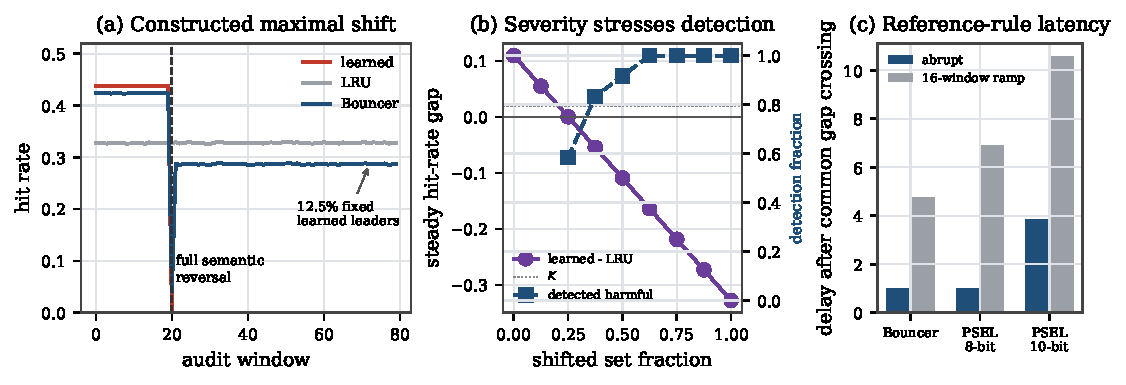
\includegraphics[width=\linewidth]{trained_characterization.pdf}
  \caption{Original operating characterization.  Panel (c) measures every bar
  from the same three-window mean gap crossing; $K$ names \system's reference,
  not a threshold implemented by PSEL.}
\end{figure}

At $p=.5$, four controlled cache/reuse configurations show that fixed $(K,H)$
does not transfer automatically: the nominal setting alarms 11/12, while a
four-way setting has $\Delta=.022$ (barely above $K$) and gates 5/12.  These are
parameter perturbations of one synthetic family, not workload diversity.

\paragraph{Representative-sampling negative control.}
Under Zipf-1.2 request weights, we reverse only the hottest eighth of sets.  They
carry 68.2\% of population request mass.  The decision-weighted follower gap is $-0.193$ but the
unweighted leader estimate is $+0.055$, so only 4/12 runs alarm.  This deliberate
premise violation gives $b_{\rm sample}$ the wrong sign; no sequential rule on
that estimate can repair it.  Pre-shift hot/cold stratification reserves one
leader/arm in the hot eighth and seven in the cold stratum.  Weighting the two
within-stratum contrasts by follower request mass reduces mean bias to $-0.0006$
and alarms 12/12, conditional on those strata capturing the heterogeneity.

\section{Secrecy and threat-model boundary}

Secrecy is unnecessary for the benign shift above.  Against an adaptive workload,
the longer artifact assumes leader identities are unobservable and evaluates
synthetic mimicry and partial leakage.  Static cache sets can in principle be
localized by set-discovery and side-channel techniques
\citep{osvik2006cache,liu2015llc}; fixed leaders therefore provide no production
security claim.  Rekeying improves freshness but can erase stateful policy
contrast, exactly as the ChampSim replacement result shows.  A deployable design
must state its adversary, concealment mechanism, rekey schedule, and warm-state
strategy; this workshop experiment supplies none of those four validations.

\begin{table}[h]
\caption{Evidence map.  Each evaluation answers a different question.}
\label{tab:evidence}
\centering
\small
\begin{tabular}{@{}p{0.20\linewidth}p{0.30\linewidth}p{0.42\linewidth}@{}}
\toprule
Evidence & Strength & Deliberate boundary \\
\midrule
Trained trace replay & Fitted controller; 12 seeded concept shifts & Controlled
workload, hit rate rather than IPC \\
Synthetic harness & Known competence, adaptive attacks, exact claim checks &
Parametric reward model \\
ChampSim/SPEC & Cycle-level execution and real cache state & Boundary study;
committed logs, no clean learned-controller validation \\
\bottomrule
\end{tabular}
\end{table}

\section{Expected-floor proof skeleton}
\label{app:theory}

Let $R_T=\sum_{w=1}^T(\bar r_w^{\pizero}-\bar r_w^{\system})$.  Split windows
into three disjoint charges.  During fully open harmful windows, bounded reward
charges at most $\rmax$ per window; the assumed expected count is
$N_{\rm ep}D$.  After gating, each harmful decision remains on $C$ only through
the audit exposure.  Under the bound's separate fresh-sampling premise,
conditional on traffic and history, a hidden uniform draw gives every set
marginal exposure at most $\phi$, so linearity of expectation charges at most
$\phi T_{\rm harm}\rmax$ without requiring independent traffic.
Finally, the expected number of false alarms is at most $\alpha T$, and each
episode costs at most $c_{\rm sw}$.  Summing the three charges yields
Equation~\ref{eq:floor}; windows where $C$ outperforms $\pizero$ contribute
nonpositive regret and may be discarded.  The premise $D$ includes both initial
detection and any false re-trust.  Only the exposure term has a separate
high-probability refinement in the full artifact.

The CUSUM used here is a score process, not a likelihood-ratio CUSUM with known
pre- and post-change distributions.  Classical Page/Lorden results therefore do
not turn the chosen $(K,H)$ into an exact false-alarm guarantee under dependent
leader rewards.  Accordingly, $D$ and $\alpha$ in Equation~\ref{eq:floor} remain
assumed or separately measured inputs.  An anytime-valid replacement would also
require explicit martingale or exchangeability conditions; time-uniformity alone
does not repair a biased estimand.

\section{Reproduction and claim ownership}

Run \texttt{./run\_ml4sys.sh}.  It regenerates the training/evaluation JSON files
and figures, checks 61 claims and boundary values, compiles this PDF, and verifies
that the main text ends by page four and references begin on page five.  All random generators
are explicitly seeded.  The trained experiment requires NumPy and Matplotlib;
the repository pins the complete environment.  The full synthetic and ChampSim
artifact remains available through \texttt{./run\_all.sh}; the latter rebuilds
figures from committed simulator logs and does not rerun every SPEC simulation.

\end{document}
